\chapter{A Review of Methods To Date}

The GALAH survey selection function is defined by simple magnitude and Galactic latitude limits \citep{Martell+2017}, and hence is not biased towards any particular stellar properties. As a result, it is expected that a majority of spectra are "typical", reflecting the underlying Galactic stellar population. This places a constraint on the techniques that can be used to identify uncommon stars, such as those exhibiting emission-line spectra. Whatever methods employed, whether manual or automated, must be adapted to detect anomalies or outliers in data—for e.g., emission-line spectra— and separate them from more typical spectra. In this work, identifying emission-line spectra in large scale surveys is presented as a pre-processing step to classification and forms a critical step in the novel method presented in Chapter 6. This chapter presents essential background material and a review of methods that have been used in the past to identify H$\alpha$ emission-line spectra, both for smaller-scale sets of observations during the latter half of the 20th century, as well as large-scale surveys in the early 21st century. These methods have also been placed in the context of their importance in the identification and classification of P Cygni, inverse P Cygni and other types of emission-line stellar spectra.

\section{A Historical Perspective}
Chapter 1 introduced the work of \citet{1953PDAO....9....1B}, who pioneered the study of emission-line stars in the 20th century. The work was manual and time consuming, and took the researcher literally decades to compile, with the assistance of a team that included secretaries and draftspeople. In spite of these efforts, the catalogue of data compiled in 1953 was small by modern standards. An in-depth literature search did not reveal further studies focused on identifying and classifying emission-line stars until several decades later, possibly due to the significant labour required to carry out these projects in the absence of modern data mining methods. 

In 1993, an atlas of high-resolution line profiles with H$\alpha$ emission-line spectra was published by \citet{van1993atlas}. The authors noted that the radial velocities of the 59 emission lines considered were generally red-shifted compared to the underlying stellar velocities. They provide a classification scheme for H$\alpha$ spectra based on emission-line morphology, devised entirely by using manual methods. More specifically, direct visual inspection and measurements of the width and shape of the line profile were used to classify these spectra, with wind velocity dispersion outside the primary disk of the star used to determine the membership of spectra in each class.

\begin{figure}[!htb]
\centering
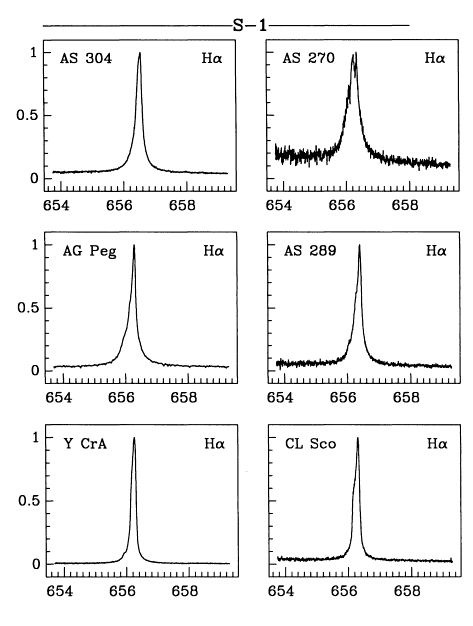
\includegraphics[scale=0.75]{figures/van winckel class.png}
\caption{Sample spectra from sub-type S1 as classified by \citet{van1993atlas}.}
\end{figure}

\begin{figure}[!htb]
\centering
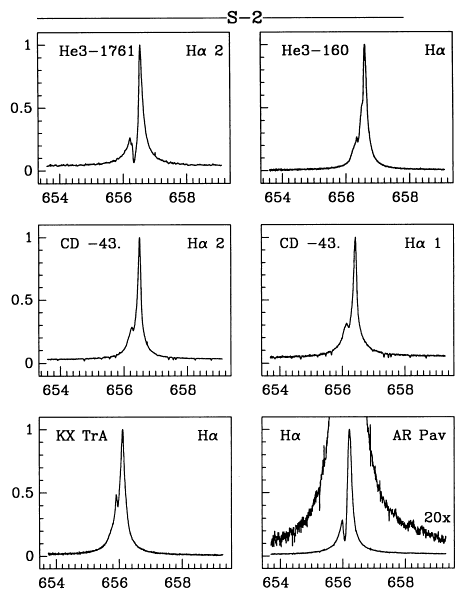
\includegraphics[scale=0.75]{figures/van.png}
\caption{Sample spectra from sub-type S2 as classified by \citet{van1993atlas}.}
\end{figure}

A few of the classes identified by the authors include sub-type S1, which displays narrow emission lines with no prominent absorption; sub-type S2, which shows a clear absorption feature superimposed on a broad emission feature; and sub-type S3, which shows a strong absorption feature reaching at least the continuum level. Stars in sub-type S3 also have the smallest wind velocity dispersions, illustrating the relationship between the morphology of the spectra and the physical processes that generate them.

\begin{figure}[!htb]
\centering
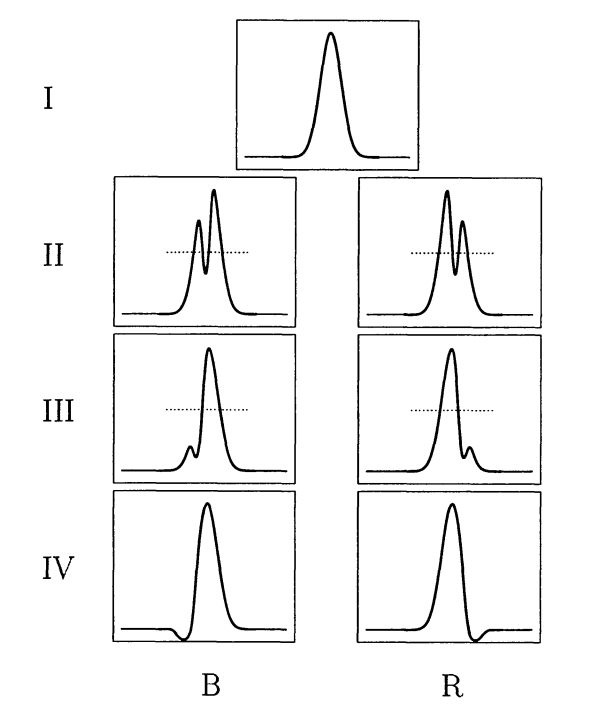
\includegraphics[scale=1]{figures/reipurth classes.png}
\caption{The morphology based classification scheme proposed by \citet{reipurth1996halpha} (reproduced). Depending on the location of the primary peak in relation to the secondary peak, the letters B and R—or blueshifted and redshifted, respectively—were appended to the Roman numerals.}
\end{figure}

Following on three years later, \citet{reipurth1996halpha} studied the H$\alpha$ emission-line profiles of pre-main sequence stars using manual methods. In addition to identifying T Tauri stars and Ae\symbol{92}Be stars using high resolution data (R$\sim$50,000), the study focused on the morphological properties of the spectra of P Cygni stars, as well as the physical processes that generate them. The study noted the discovery of complex morphological profiles among the T Tauri, Ae\symbol{92}Be and P Cygni star classes, for which the authors proposed a two-dimensional classification scheme based on the relative height of a secondary peak compared to the primary peak, and whether the absorption line is blue- or redshifted. In their observed sample, the authors noted the classification of 25\% symmetric profiles, 49\% blueshifted absorption profiles and 5\% P-Cygni profiles, with some 21\% falling into the redshifted absorption category. In addition to this morphological classification, the authors also measured stellar wind velocities, with some stars recording extremely high velocities of $\sim$900km/s. 

The classification of P Cygni stars in \citet{reipurth1996halpha} follows the scheme proposed by \citet{1953PDAO....9....1B}. The authors also compared observational data to models in the literature, particularly models that constrain mass, radii and photospheric temperatures, although no specific model details for P Cygni stars were provided. Further catalogues of H$\alpha$ emission-line stars were produced by \citet{kohoutek1999catalogue}. These catalogues contain 98 identified emission-line stars in the Northern Milky Way, but do not specifically identify P Cygni stars or inverse P Cygni stars.

Working with data from NGC 6611, \citet{bonito2013spectroscopic} noted that, for stars surrounded by active disks, the morphology of  emission lines could fall into categories such as symmetric with broad wings, asymmetric and, in extreme cases, P Cygni and inverse P Cygni. The authors used the classification scheme proposed by \citet{reipurth1996halpha} mentioned above, adhering to the type I - IV scheme with B and R suffixes to denote blueshifted and redshifted emission lines respectively.

 \citet{traven2015gaia} presented a catalogue of H$\alpha$ emission-line stars identified in the Gaia-ESO survey. This survey's selection function was biased towards young open clusters, and consequently the authors noted a relatively large proportion of H$\alpha$ emission-line spectra in their data: 3765 emission-line stars were identified from a sample of 22,035 spectra. This work is notable as it uses a combination of empirical rules and automated methods like spectral fitting to sort the H$\alpha$ emission-line spectra into eight distinct morphological categories. These include, single–component emission, emission blend, sharp emission peaks, double emission, P-Cygni, inverted P-Cygni, self–absorption, and emission in absorption. This work was briefly introduced in Chapter 1.  

\begin{figure}[!htb]
\centering
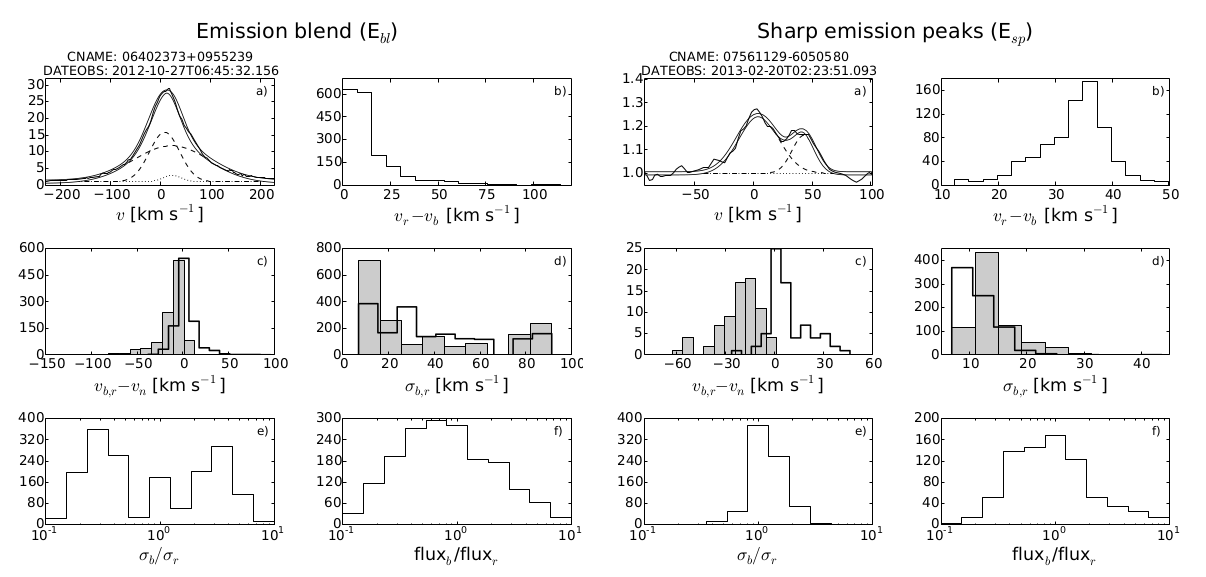
\includegraphics[scale=.47]{figures/gaia eso1.png}
\caption{Classes of emission-line spectra identified in the Gaia-ESO Survey. Reproduced from \citet{traven2015gaia}.}
\end{figure}

\begin{figure}[!htb]
\centering
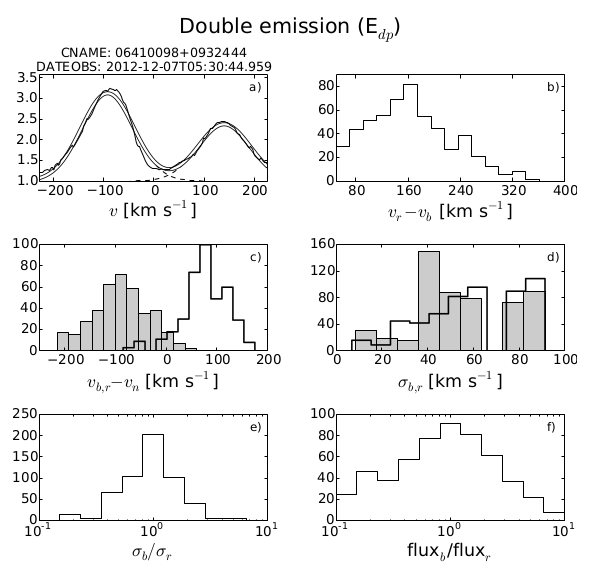
\includegraphics[scale=.85]{figures/gaia eso2.png}
\caption{Classes of emission-line spectra identified in the Gaia-ESO Survey. Reproduced from \citet{traven2015gaia}.}
\end{figure}

The Gaia-ESO survey conducted repeat observations of about half the identified H$\alpha$ emission-line stars, and hence the authors were able to comment on the temporal variability of these stars. The conclusion was that, while some morphological categories exhibited stability of their spectral profiles over time, P-Cygni and self-absorption profiles may not. Supplementary information on these spectra from cross-matches to SIMBAD, VizieR and ADS were also provided. In addition to these data, the authors  provided wind velocity estimates based on a curve fitting procedure. In their discussion, the authors noted that the identification, classification and characterisation of emission-line stars can be valuable for automated pipelines in large surveys, where they can pinpoint outliers when calculating general stellar properties and abundances for the larger sample. Additionally, they note that the stars thus identified can be used for studies of star formation processes, interacting binaries and related fields of stellar physics. 

Several conclusions can be drawn from this historical perspective: 

\begin{enumerate}
\item These methods relied exclusively on visual inspection of spectra and manual methods to identify and/or classify H$\alpha$ emission-line spectra. While this may have been a suitable approach in the past, it is extremely challenging to extend and scale these methods to data sets generated by million star all-sky surveys in the present day.
\item As noted in Chapter 1, a variety of spectral morphologies are believed to be generated by distinct physical phenomena linked to stellar disks and the gas that surrounds them. Thus morphology-based classification approaches, as demonstrated by \citet{reipurth1996halpha} and \citet{1953PDAO....9....1B}, are crucial to developing a greater understanding of stellar evolution and dynamics.
\item Finally, these studies identified P Cygni and inverse P Cygni (among other classes of spectra) as a subset of H$\alpha$ emission-line spectra. The current work takes this fact to its logical conclusion, i.e., the probability (and efficiency) of identifying P Cygni and inverse P Cygni spectra can be increased if the search space and feature space of the raw data is reduced from a complete survey data set \citep[e.g., the complete GALAH survey DR3 catalogue;][]{buder2021galah+} to a much narrower subset of H$\alpha$ emission-line spectra during pre-processing. 
\end{enumerate}

\section{Recent Developments}
The increase in data availability via large-scale spectroscopic surveys has necessitated the use of automated identification and classification methods. In recent years these methods have included a veriety of statistical analysis and machine learning techniques. In general, machine learning approaches can fall into two categories: supervised and unsupervised learning. The former relies on the availability of a suitably robust set of training examples, while the latter attempts to generalise and learn from unlabelled data \citep{hastie2009elements}. 

While a full discussion and review of machine learning techniques is beyond the scope of this thesis, the methods that are relevant to this work are presented in subsequent chapters, with Chapter 4 in particular presenting a more detailed discussion on the relevant methods. The following section reviews four recent studies that use machine learning to identify spectra in large surveys, and discusses their strengths and limitations.

\subsection{Applying K-means Clustering Directly on Data from APOGEE}
The goal of k-means clustering is to partition a set of observations into a predefined set of clusters. Each observation would belong to a cluster with the nearest mean, which serves as the centroid or prototype of the cluster \citep{macqueen1967some}. Formally, given a set of $n$ observations such as \(x_1,x_2,...,x_n\), where each observation is a $d$-dimensional vector, the algorithm will partition the $n$ observations into $k$ sets $S=\{S_1,S_2,...,S_k\}$, such that the intra-cluster variance is minimised. This objective can be represented as:

\begin{equation}
{\underset {\mathbf {S} }{\operatorname {arg\,min} }}\sum _{i=1}^{k}\sum _{\mathbf {x} \in S_{i}}\left\|\mathbf {x} -{\boldsymbol {\mu }}_{i}\right\|^{2}={\underset {\mathbf {S} }{\operatorname {arg\,min} }}\sum _{i=1}^{k}|S_{i}|\operatorname {Var} S_{i}
\end{equation}

where $\mu_i$ is the mean of the points in $S_i$. 

Using the identity,

\begin{equation}
    |S_{i}|\sum _{\mathbf {x} \in S_{i}}\left\|\mathbf {x} -{\boldsymbol {\mu }}_{i}\right\|^{2}=\sum _{\mathbf {x} \neq \mathbf {y} \in S_{i}}\left\|\mathbf {x} -\mathbf {y} \right\|^{2}
\end{equation}

it can be shown that this is equivalent to minimising the pairwise squared deviations of points belonging to the same cluster.

\begin{equation}
{\underset {\mathbf {S} }{\operatorname {arg\,min} }}\sum _{i=1}^{k}\,{\frac {1}{|S_{i}|}}\,\sum _{\mathbf {x} ,\mathbf {y} \in S_{i}}\left\|\mathbf {x} -\mathbf {y} \right\|^{2}
\end{equation}

This method was used on high-resolution APOGEE infrared spectroscopic data (R$\sim$22,500), taken as part of the Sloan Digital Sky Survey (SDSS) \citep{eisenstein2001spectroscopic, blanton2017sloan}. In the absence of labelled training samples in the APOGEE survey, \citet{garcia2018machine} used k-means to cluster similar spectra into distinct groups: each spectrum produced by APOGEE was treated as a $d$-dimensional vector; the number of observations $n$ was the number of spectra generated by APOGEE, which was approximately 150,000; and $k$ was set to 50, presumably by a process of trial and error. The authors noted that they were able to separate dwarfs, sub-giants, red clump and red giant branch stars using this approach. The authors also commented that the approach is sensitive to initialisation, and thus sensitive to the number of clusters, $k$. One major limitation of this approach is that a discrete classification in flux space does not result in a neat organisation in parameter space, which implies that the authors were not able to link spectral features such as spectroscopic morphologies to the machine learning parameter space. The other limitation is the manual sorting of clusters that reduced the number of clusters from 50 to 9. This implies that certain spectra were incorrectly clustered by the k-means algorithm. Notably, the authors were unable to cluster emission-line spectra using this method. 

The primary conclusion that can be drawn from this work is that k-means clustering, while robust on more traditional machine learning tasks, may perform poorly if it is used to cluster and ultimately classify morphologically-similar spectra such as P Cygni, inverse P Cygni and other emission-line classes traditionally identified using manual methods. A method that relates flux space, and consequently the morphology of the spectrum to a parameter space may perform better than k-means. 

\subsection{Combining Machine Learning and Manual Methods on Data from the LAMOST Survey}

The LAMOST survey is a low-resolution spectroscopic survey with 10 million Milky Way stars as potential survey spectra. \citet{zhang2021catalog} were able to use a training and test set (labelled spectra) comprising of 5915 samples for spectral classification. This training set was based on data released by \citet{hou2016catalog}, who developed the data set by using a combination of empirical rules and visual examination of 10,000 LAMOST spectra. The labelled data, including seven P Cygni and inverse P Cygni spectra identified by \citet{hou2016catalog} was used by \citet{zhang2021catalog} for supervised machine learning algorithms. Ten different supervised learning methods were then applied to this data set including including KNN (K-Nearest Neighbor), RF (Random Forest), AdaBoost, Naive Bayes (MultinomialNB, GaussianNB, BernoulliNB), logistic regression, SVM (Support Vector Machine) and Artificial Neural Network (Single-hidden Layer, Three-hidden Layer). A comparison of the relative performance of these different methods was not provided by the authors, and a detailed discussion of all these methods would be beyond the scope of this thesis. 

\citet{zhang2021catalog}, however, note that the k-nearest neighbour and random forest methods outperformed all other methods. These two supervised machine learning models were then applied to 498,588 spectra, resulting in 56,574 potential H$\alpha$ emission-line spectra. These spectra were then visually inspected, with a final candidate list of 30,048 H$\alpha$ emission-line spectra. Despite the use of a number of machine learning methods, the authors fell back on manual visual inspection of spectra in building the training set, and during the classification of the identified potential H$\alpha$ emission-line spectra. Thus it is clear that machine learning methods must be aligned with the desired end goals such that the work does not ultimately need to fall back on using manual methods.

\subsection{Dimensionality Reduction in Action: Using t-SNE to Classify GALAH Spectra}

Conducting computational operations such as clustering and classification on a higher dimensional vector space of size $\sim$4500 can be challenging as it introduces significant computational overheads. In addition to the so-called curse of dimensionality, which will be detailed in Chapter 3, researchers would also face practical limitations due to the computational intractability of working on higher-dimensional vector spaces. It would therefore be helpful to transform complex data sets from a high-dimensional space to a low-dimensional space while ensuring that meaningful features of the original data are preserved. In the case of P Cygni and inverse P Cygni spectra, these meaningful properties would presumably include some information about the morphology of the spectrum, although a reduction method may not guarantee this.

Principal component analysis (PCA) is arguably the most well-known dimensionality reduction method. However, PCA may not be suitable in the context of GALAH DR1, and certainly GALAH DR3, since these data sets are arguably biased towards {\em non}-emission-line spectra. A PCA-led approach may select features that represent the absorption-line, while emission-line features are ignored. This hints at a possible outlier or anomaly detection-based approach to emission-line spectrum identification. This idea is revisited in Chapter 6.

More recent and novel dimensionality reduction methods such as t-distributed stochastic neighbour embedding (t-SNE) \citep{van2008visualizing} have been used on spectral data from GALAH DR1 \citep{traven2017galah}. A stellar spectrum of vector length $d$ (a wavelength grid of size $d$) can be used to create a vector space of dimensionality equal to $d$. In the case of GALAH DR1 this value is $\sim$4500. Given a vector of size $d$, the application of the t-SNE algorithm will project this vector space onto a two-dimensional vector space. The distances between data points on this two-dimensional vector space can then be used to cluster similar data points into similar groups using a variety of popular clustering methods such as DBSCAN \citep{ester1996density} or HDBSCAN \citep{campello2013density}. A detailed discussion of this method and its suitability to this work is presented in Chapter 5.

\begin{figure}[!htb]
\centering
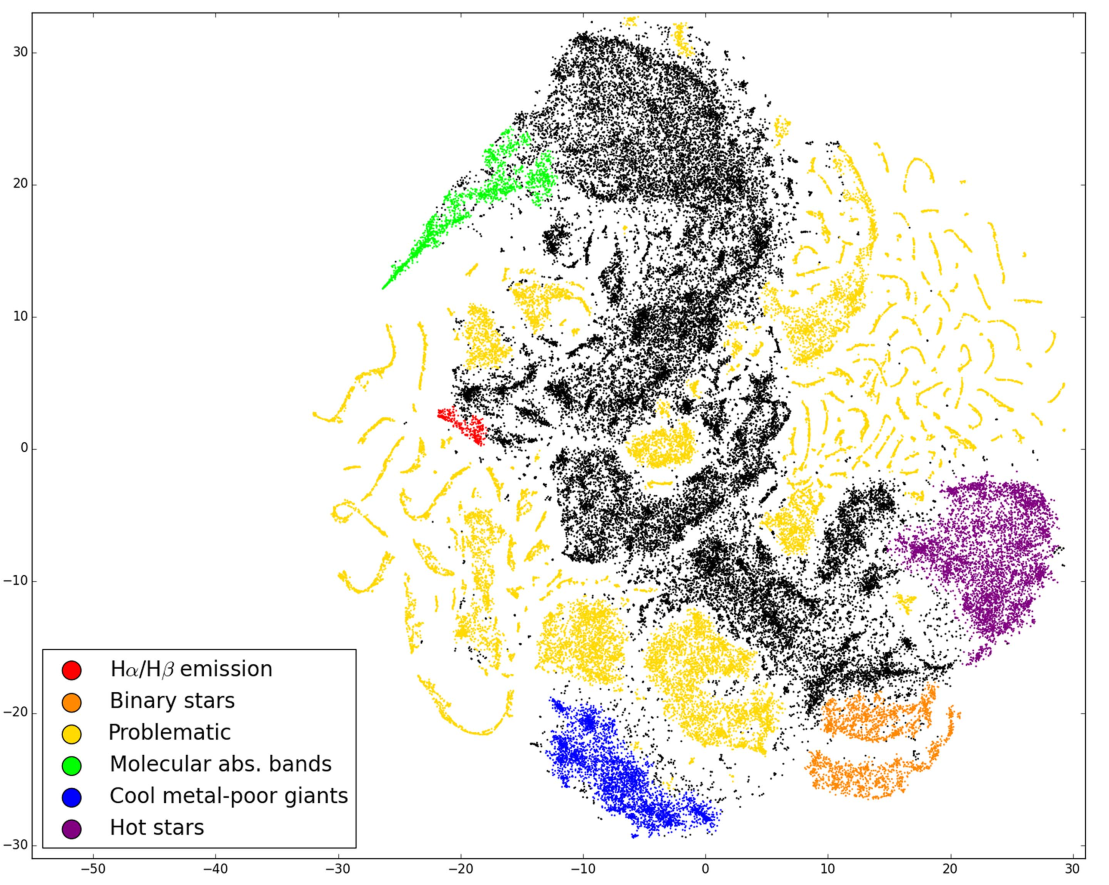
\includegraphics[scale=0.36]{figures/tsne traven.png}
\caption{The t-SNE plot for GALAH DR1 with classified regions, reproduced from \citet{traven2017galah}. The x and y axes do not have a direct physical meaning but serve as spanning vectors for the two-dimensional space.}
\label{fig2.6}
\end{figure}

Using this method, Traven et al. classified six distinct stellar types and identified H$\alpha$ and H$\beta$ emission-line spectra in GALAH DR1. These spectra were further examined and 18 P Cygni spectra were identified. The identification of P Cygni spectra was a sub-component of a broader study of stellar types in GALAH DR1. The authors noted that the number identified was lower than expected, which implies that there is significant scope to develop methods capable of detecting a larger number of emission-line stars in the GALAH survey. Crucially, this method was not able to separate P Cygni spectra from double peaked spectra, emission superimposed on absorption and other types of emission-line spectra. When examining the t-SNE plot (Figure \ref{fig2.6}), it is clear that the authors were not able to separate H$\alpha$ emission-line stars as a distinct cluster from the unclassified region (black) but rather fell back on manual tagging of this region on the projection space. 

Dimensionality reduction can overcome problems such as computational intractability but this should ideally not be at the cost of information losses related to the morphology of the spectrum. Since these morphologies uniquely identify the spectral types, a significant loss of this information will lead to poor classification performance. This point is revisited in detail in Chapter 5, providing examples using t-SNE where this type of information loss may have occurred.

\subsection{Neural Networks as Anomaly Detectors: Using an Autoencoder on Data from GALAH and Other Surveys}

In contrast to t-SNE, \citet{vcotar2021galah} introduced an anomaly detection-based approach to identify emission-line stars, the performance of which was a significant improvement over the t-SNE based method described above. This method used an autoencoder (AE), which is a type of artificial neural network (ANN) that takes input data and reduces it to a pre-selected number of "latent features" that inhabit a low-dimensional vector space, known as the latent space. The latent space can capture important features that exist in the original $d$-dimensional vector space. By processing $n$ samples of $d$-dimensional vectors, the autoencoder can then learn the latent space representation of the higher dimensional features. This is known as encoding. In the next portion of the network, the network then attempts to recover the original data from the latent vector space. The process that reduces a $d$-dimensional vector and vector space to a vector space of size $p$<$d$ is a dimensionality-reduction method similar to PCA or t-SNE. The portion of the network that takes a $p$-dimensional vector from the latent space and then projects it back to a $d$-dimensional vector space is essentially the inverse process of the dimensionality reduction procedure. This component is known as a decoder. Since the original data are generated from the latent space, autoencoders fall into a class of ANNs called generative models (generative ANNs). Note that the latent space for an autoencoder is discrete. (ANNs that can generate {\em continuous} latent spaces in this manner are known as variational autoencoders—VAEs—but are beyond the scope of this work.) 

Autoencoders are widely used in anomaly detection applications \citep{sakurada2014anomaly} and can be suitably adapted to detect atypical spectra from survey data that contain a majority of typical spectra. If the autoencoder model is trained on non-anomalous data ("normal" data), the model will learn the latent space representation of non-anomalous data. Subsequently, if an anomalous data point is passed through the model, the autoencoder will attempt to generate these data from the latent space representation it has learned. Since the learned model was trained on {\em non}-anomalous data, the autoencoder will generate an inaccurate representation of the anomalous data. This leads to a prediction error, which can be used as a flag to detect time-series as well as non time-series anomalies in data.

As noted previously, the GALAH survey is a general all-sky survey that can be expected to generate a significantly higher proportion of non-anomalous spectra—specifically, since it is not biased towards young, violent, hot stars or stellar nurseries, we expect the vast majority of spectra to show "typical" (non-anomalous) stellar H$\alpha$ line profiles, i.e., an absorption feature. In this regime, an H$\alpha$ emission-line, and consequently, P Cygni and inverse P Cygni spectra are rare and anomalous. If an autoencoder is trained on "normal looking" spectra which do not show emission lines near H$\alpha$, it can be made sensitive to H$\alpha$ emission-line spectra. 

\begin{figure}[!htb]
\centering
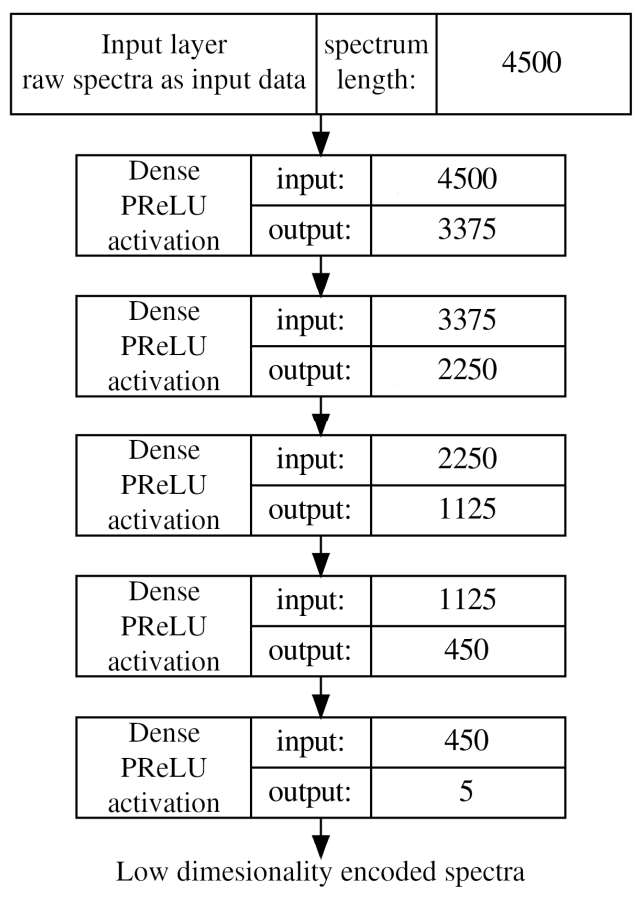
\includegraphics[scale=0.45]{figures/autoencoder.png}
\caption{An autoencoder architecture capable of detecting H$\alpha$ emission-line spectra in GALAH survey data. Reproduced from \citet{vcotar2021galah}.}
\label{fig2.7}
\end{figure}

This method was used by \citet{vcotar2021galah} to detect H$\alpha$ emission-line spectra in GALAH survey data. The authors chose a network architecture that reduces a $d$-dimensional GALAH spectrum to a $p$-dimensional latent space representation; here, $d$ = 4500, while $p$ = 5. Presumably, $p$ was set to 5 to potentially capture the primary stellar parameters and represent them within the latent space. The intervening layers and the final architecture capable of detecting H$\alpha$ emission-line spectra are presented in Figure \ref{fig2.7}. The authors did not further classify P Cygni, inverse P Cygni or other types of emission-line spectra using this method. 

\section{Concluding Remarks}

It is clear from the review presented here that, given the scale of many contemporary astronomical data sets, modern work should rely heavily on automated methods when identifying atypical spectra such as those of emission-line stars. Attempts have been made at using machine learning methods to tackle this problem over the last five years with varying levels of success. If labelled data are available, supervised machine learning methods can be applied as in the case of \citet{zhang2021catalog}. However, these methods must be applied appropriately if progress is to made with regards to relying on human beings to detect atypical spectra in large-scale surveys.

Regarding P Cygni stars and inverse P Cygni stars specifically, the literature dealing with their detection and characterisation is sparse and the available samples are few. A comprehensive catalogue of these spectra and stars does not exist at present. This can limit the use of supervised machine learning methods, and more importantly, can limit the science conducted on these spectra in the literature. Thus improvements to methods—and the introduction of novel methods—can lead to more emission-line spectra being identified and classified, which in turn can lead to new science results on these stars. 

The use of machine learning has been a relatively new development in the field. As far as can be determined from the literature, the use of t-SNE in 2017 is the first instance of applying machine learning to identify and classify H$\alpha$ emission-line spectra. However, as will be demonstrated in Chapter 5, it can be challenging to use t-SNE to classify P Cygni and inverse P Cygni spectra, among other types of objects. Dimensionality reduction methods must be chosen carefully, so as not to lose too much information with regards to the features of the emission-line spectra.

Taking an anomaly detection or outlier detection approach such as \citet{vcotar2021galah}, and using a neural network architecture such as an autoencoder can be beneficial in reducing the search space of surveys such as GALAH from the set of all spectra available to only the potential emission-line spectra. However this method cannot be used to classify particular types and sub-species of emission-line stars such as P Cygni and inverse P Cygni. Similar to dimensionality reduction, this method can reduce the complexity of the problem by allowing the researcher to focus on only the most relevant data points when attempting to identify and classify emission-line spectra. Combined with other methods, this method can serve as a pre-processing step when identifying and classifying emission-line spectra. This idea is explored more fully in Chapters 4 and 6. 

Finally, popular unsupervised machine learning methods such as k-means, as well as supervised machine learning methods such as logistic regression may not be suitable. The latter requires labeled training data which was not available for this work, and there is evidence from the literature that the former performed poorly on the task of identifying and classifying emission-line stars in a large scale spectroscopic survey \citep{garcia2018machine}. Hence these methods were not considered in this work.

